\documentclass[12pt,oneside]{sotsuken_paper}

\usepackage{listings}
\renewcommand{\lstlistingname}{mecanum}
\lstset{language=C,%
        basicstyle=\footnotesize,%
        commentstyle=\textit,%
        classoffset=1,%
        keywordstyle=\bfseries,%
	frame=tRBl,framesep=5pt,%
	showstringspaces=false,%
        numbers=left,stepnumber=1,numberstyle=\footnotesize%
	}%

% タイトル
\title{ジャイロセンサを用いたロボットの方向自動修正}
\author{平元隆顕・松村隆平}

\begin{document}
% 行間
\setlength{\baselineskip}{9truemm}

%文字間
\kanjiskip=.53zw plus 3pt minus 3pt
\xkanjiskip=.53zw plus 3pt minus 3pt

% 目次
\tableofcontents
%\newpage

% 本文

\chapter{はじめに}

	\section{研究の背景}

		\subsection{2016年度「ロボット・ニューフロンティア」ルール説明}
		2016年度に行われたNHK高専ロボコンは「ロボット・ニューフロンティア」という題目で港町から海を渡り、新大陸を目指すというものである。
		使用ロボット台数は無制限、港町で灯台を組み上げ、床に接触しないよう海を渡り、丘の上に砦を築く競技である。今年は丘に積み上げた砦の高さを競い合うものであった。図\ref{競技フィールド}はこの競技のフィールドである。

		\begin{figure}[htp]
			\begin{center}
				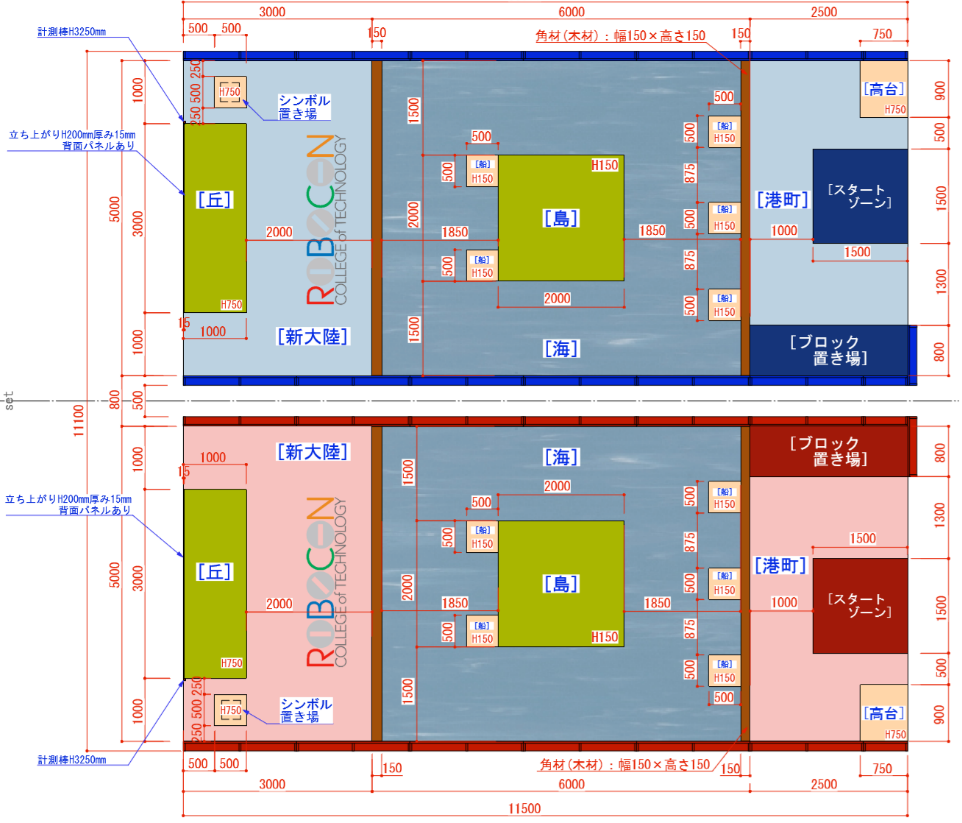
\includegraphics[width=120mm]{Image/フィールド.png}
				\caption{競技フィールド}
				\label{競技フィールド}
			\end{center}
		\end{figure}

	\section{研究の目的}
	今回ロボコン競技に使用した積み込みロボットの移動手段となっている全方向移動可能なメカナムホイールにジャイロセンサを加えることで継続的に直進を可能にする。

\chapter{メカナムホイールを採用した理由}
何故、今回のロボコンでメカナムホイールを採用したかを以下に示す。

\begin{itemize}
	\item 出題された多くの課題の中で制限時間3分は非常に短く、丘に箱を積み上げるだけでも困難になる。
	\item メカナムホイールを使用することで2輪駆動よりも圧倒的に速く課題をクリアすることができる。
\end{itemize}

	\section{二輪駆動ロボとメカナムロボの比較}
	メカナムホイールは2輪駆動よりも少ない工程で動作が可能である。例としてロボットの向きを変えずに右に移動させたい場合、2輪駆動ロボットでは90°右旋回してから前進、正面を向き直す為90°左旋回と少なくとも3工程必要となる。これがメカナムホイールの場合は横に並行移動の1工程だけで終えることができる。また、メカナムホイールは移動しながらの旋回も可能で1工程の時間の中で2工程分の動きも可能なのである。このように、メカナムホイールを用いることで2輪駆動よりも少ない工程数で時間の短縮が可能なのである。

	\section{三分間で必要とされる動き}
	メカナムホイールを使っている積み込みロボットが競技中の三分間で必要とされる動きを以下に示す。

		\subsection{箱の持ち運び}
		特定の位置に並べられている箱を持ち上げ、距離4mほど運搬する必要がある。この時の課題は箱を拾う際の位置調整である。箱は図\ref{ブロック}のように400mm×300mm×200mmで100mmの等間隔に設置されている。その100mmの間を図\ref{箱回収位置寸法}のように幅約72mmのハンドを滑り込ませ、更に側面から見た図\ref{箱回収側面位置}のように縦は中心で横が先端から約110mm前後の位置にハンドの中心がくるように配置しなければならない。そのためメカナムホイールの全方向移動による微調整が2輪駆動より有効となる。

		\begin{figure}[htp]
			\begin{center}
				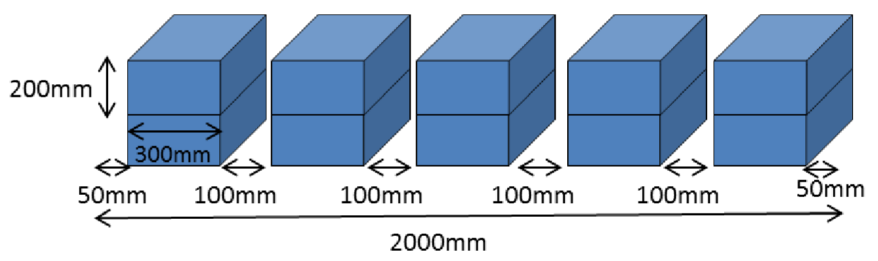
\includegraphics[width=100mm]{Image/ブロック.png}
				\caption{競技中の箱配置}
				\label{ブロック}
			\end{center}
		\end{figure}

		\begin{figure}[htp]
			\begin{center}
				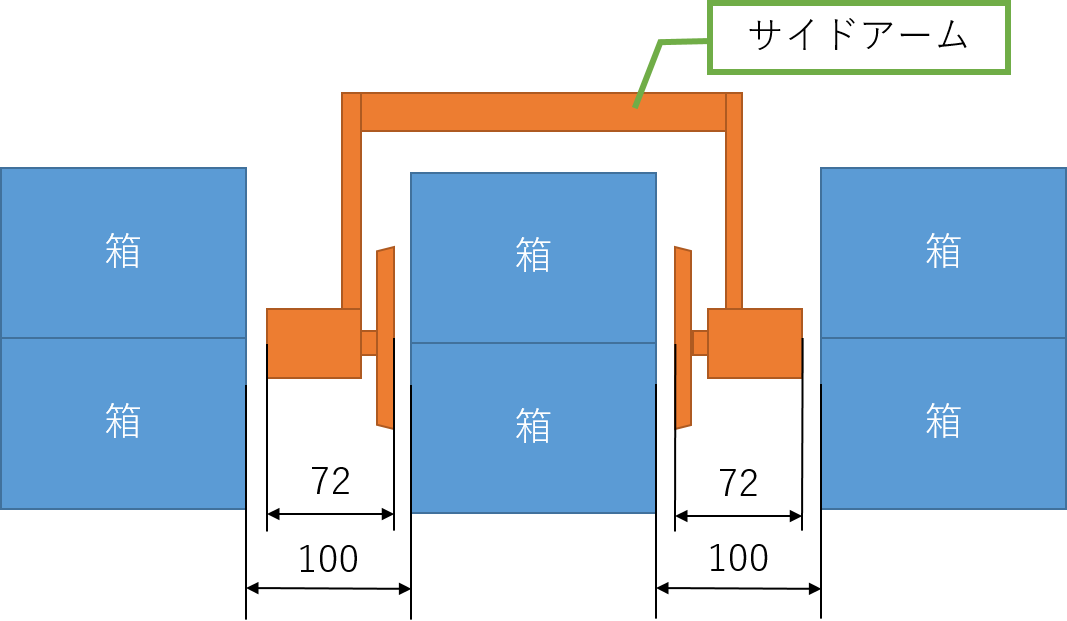
\includegraphics[width=80mm]{Image/箱回収位置寸法.png}
				\caption{箱の幅とアームの幅}
				\label{箱回収位置寸法}
			\end{center}
		\end{figure}

		\begin{figure}[htp]
			\begin{center}
				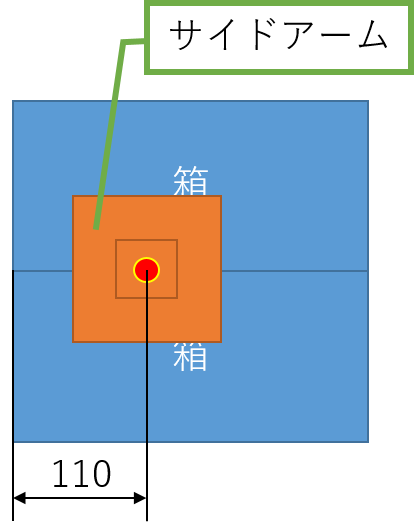
\includegraphics[width=60mm]{Image/箱回収(側面).png}
				\caption{箱回収側面位置}
				\label{箱回収側面位置}
			\end{center}
		\end{figure}

		\subsection{塔建て}
		運んだ箱を高さ750mmの台の上に持ち上げて、下段が大きく上段が小さくピラミッド型のように組み立てる。これは「高台」と「丘」によって異なり、「高台」では図\ref{高台の箱積}のように2列1列1列の順に組み立てる。「丘」では図\ref{丘の箱積}のように下段が上段よりも両側25mm程大きければいくらでも積んで良いとなっている。
		製作した積み込みロボットは「丘」であれば動かずに積み上げることができる。だが「高台」の場合は1列に2段積み上げる必要があるため真横に並行移動できると時間短縮になる。

		\begin{figure}[htp]
			\begin{center}
				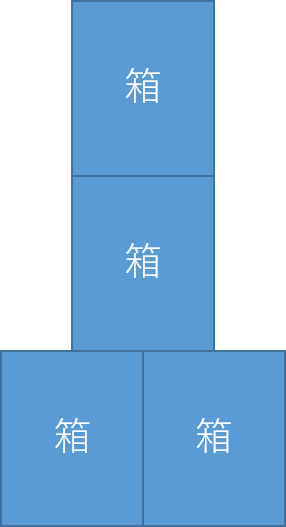
\includegraphics[width=30mm]{Image/高台箱積.png}
				\caption{高台の箱積}
				\label{高台の箱積}
			\end{center}
		\end{figure}

		\begin{figure}[htp]
			\begin{center}
				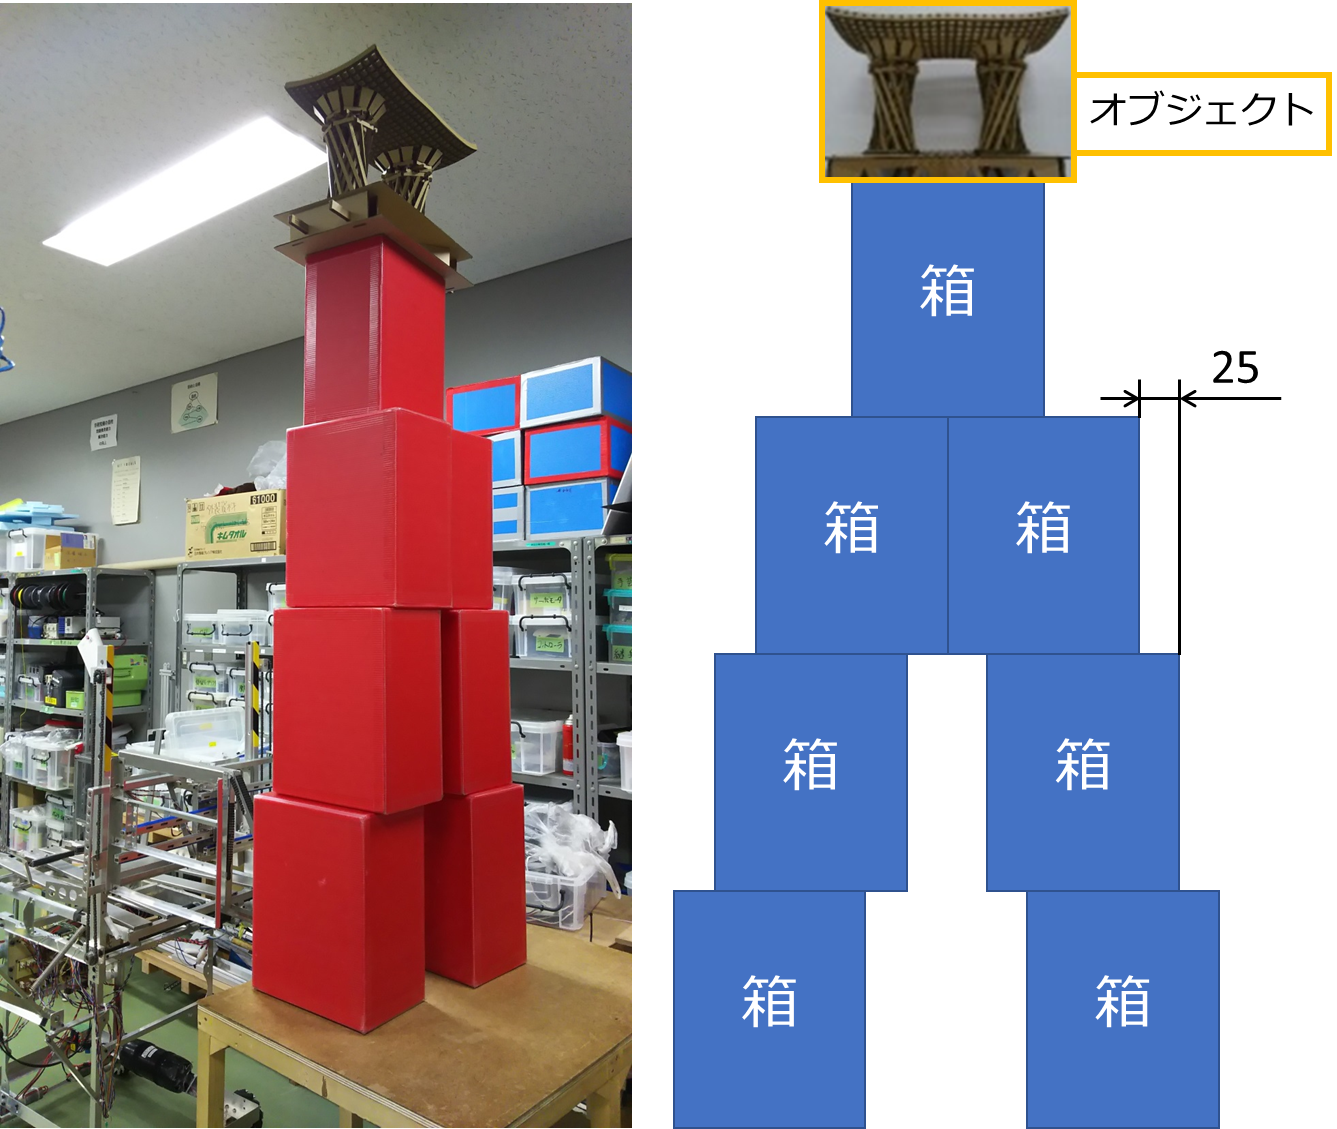
\includegraphics[width=80mm]{Image/丘の箱積.png}
				\caption{丘の箱積}
				\label{丘の箱積}
			\end{center}
		\end{figure}

		\subsection{橋渡り}
		架橋ロボが設置した橋の上を渡るが、その橋に侵入する際に橋幅約80mmでタイヤ2輪同時侵入の位置調整は難しく、2輪駆動だと時間が掛かる。そのため、並行移動できるメカナムホイールは2輪駆動よりスムーズに位置調整が可能である。

		\subsection{オブジェクトの持ち運び}
		丘の左または右に設置されているオブジェクト置き場からオブジェクトの鼓門を持ち運び砦のてっぺんに設置する、この際2輪駆動では旋回を何度も必要となるため、並行移動ができるメカナムホイールが有効的である。

\chapter{メカナムホイールの説明}
メカナムホイールとは、一般の自動車と同じように4輪1セットで使用するが、相違点がいくつか存在する。今回は、形状が特殊であること、向きによって取り付ける場所が決定されていること、各車輪に異なる回転数を与えることで任意の方向に移動可能であることの3点を説明する。外見は樽状のタイヤが外周を覆うようにして取り付けられている。また、このタイヤの回転軸は水平・垂直方向から45度傾いている。

	\section{メカナムホイールの外見}
	外見は樽状のタイヤが外周を覆うようにして取り付けられており、このタイヤの回転軸は車輪の水平・垂直方向から図\ref{角度}のように45度傾いている。

	\begin{figure}[htp]
		\begin{center}
			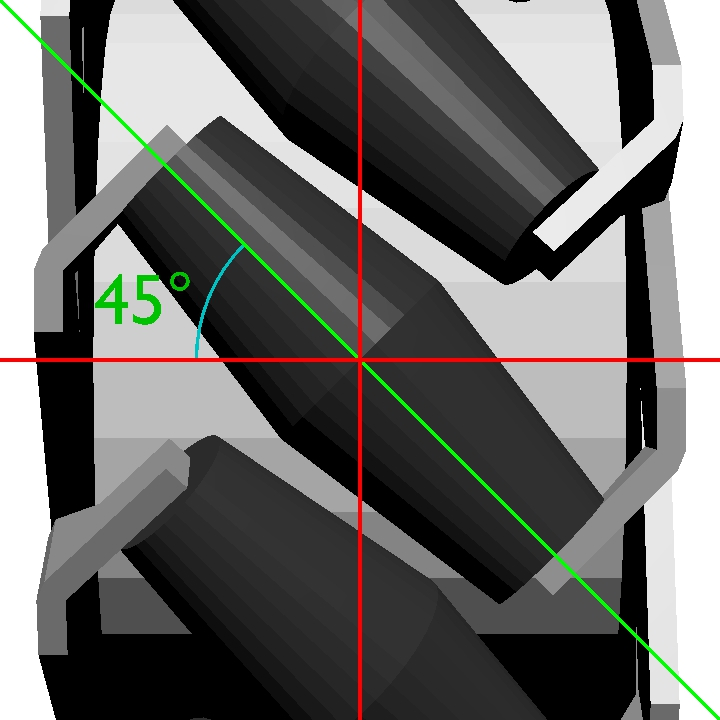
\includegraphics[width=60mm]{Image/角度.jpg}
			\caption{タイヤの角度}
			\label{角度}
		\end{center}
	\end{figure}

	\section{ホイールの向きと組み合わせ}
	メカナムホイールには向きがあり、これらを正しく取り付けなければ正常に動作しない。図\ref{対角}のように各車輪に対して縦と横方向に存在する車輪は互いに逆向きの関係であるが、対角に存在する車輪は同じ向きとなる。今回では図\ref{角度}の向きを順方向として扱い、メカナムホイールごとに番号を振り分けた場合、1番と4番は順方向、2番と3番は逆方向となる。

	\begin{figure}[htp]
		\begin{center}
			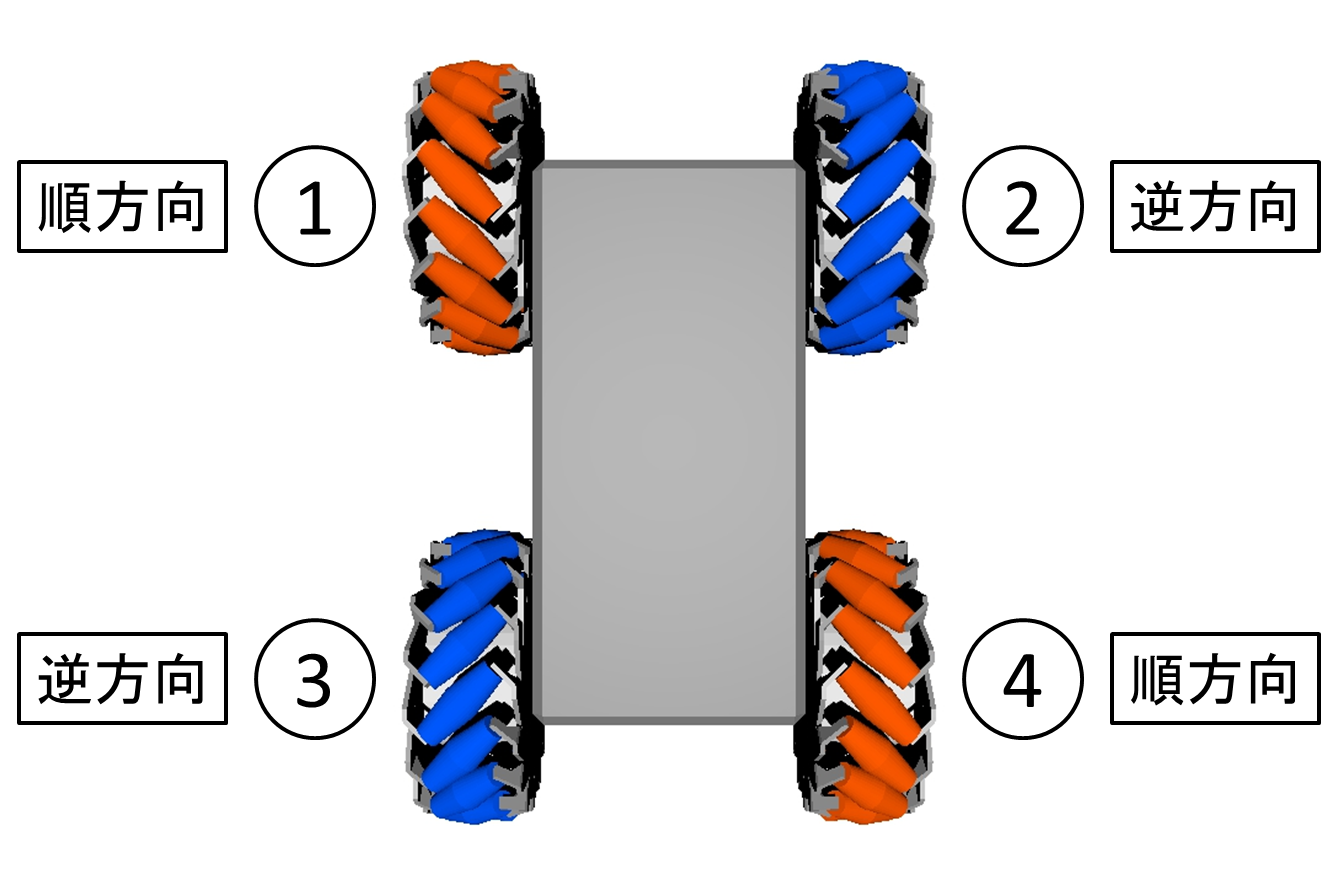
\includegraphics[width=100mm]{Image/対角.png}
			\caption{組み合わせ}
			\label{対角}
		\end{center}
	\end{figure}

	\section{各動作}
	ここではホイール単体の動作と四輪を組み合わせた全体の動作を説明する。

		\subsection{単体の動作}
		静止した状態では地面に接触しているタイヤの回転方向に進むが、回転時ではその逆方向に移動する。図\ref{回転系}は地面から見たそれぞれの車輪の動きを示している。

		\begin{figure}[htb]
			\begin{center}
				\begin{tabular}{c}
					\begin{minipage}{0.5\hsize}
						\begin{center}
							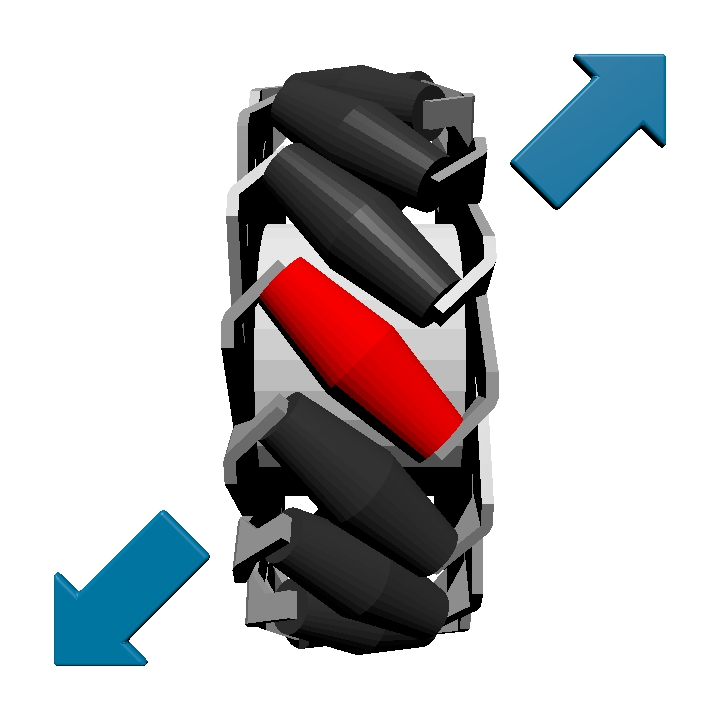
\includegraphics[width=60mm]{Image/無回転.jpg}
							\\(a)無回転
						\end{center}
					\end{minipage}
					\begin{minipage}{0.5\hsize}
						\begin{center}
							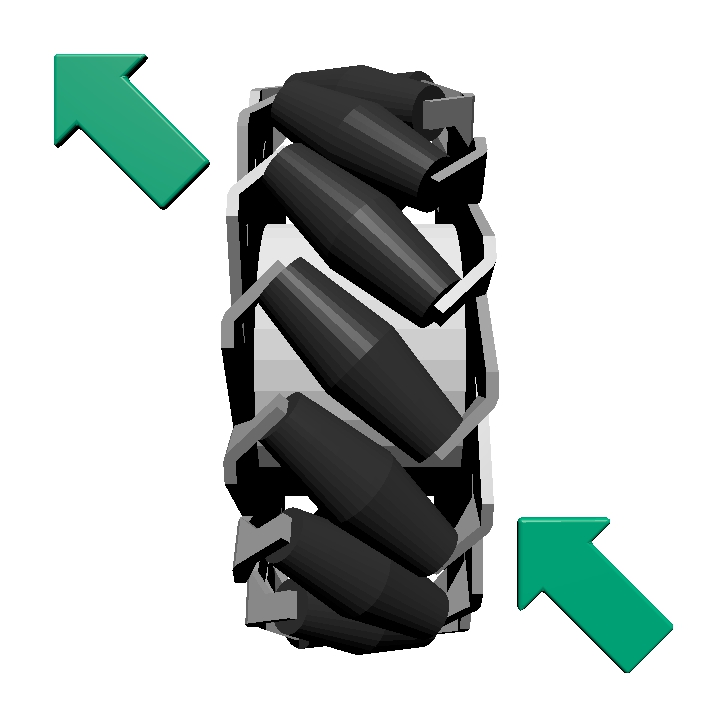
\includegraphics[width=60mm]{Image/回転.jpg}
							\\(b)回転
						\end{center}
					\end{minipage}
				\end{tabular}
				\caption{地面から見た車輪の動き}
				\label{回転系}
			\end{center}
		\end{figure}

		\subsection{全体の動作}
		四輪の状態での動作は車輪の回転によって発生するX方向もしくはY方向のベクトルを互いに打ち消し合うことで、図\ref{移動系}に示すように任意の方向に並行移動することができる。

		\begin{figure}[htb]
			\begin{center}
				\begin{tabular}{c}
					\begin{minipage}{0.33\hsize}
						\begin{center}
							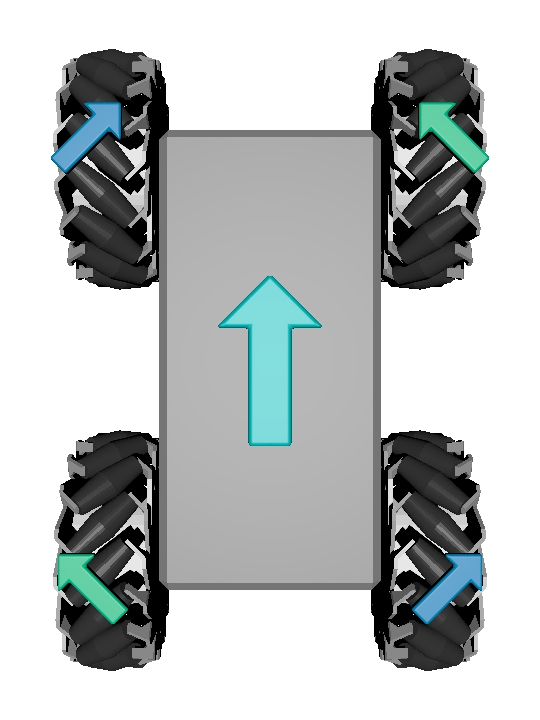
\includegraphics[width=40mm]{Image/ロボット1}
							\\(a)前進
						\end{center}
						\begin{center}
							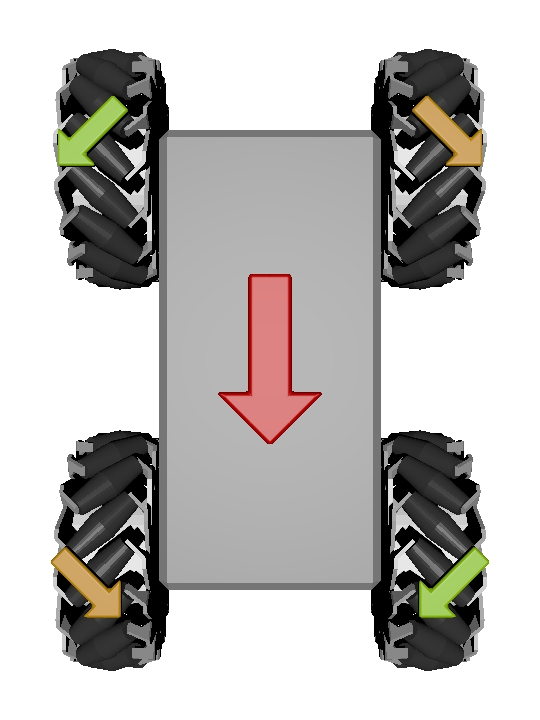
\includegraphics[width=40mm]{Image/ロボット2}
							\\(b)後進
						\end{center}
					\end{minipage}
					\begin{minipage}{0.33\hsize}
						\begin{center}
							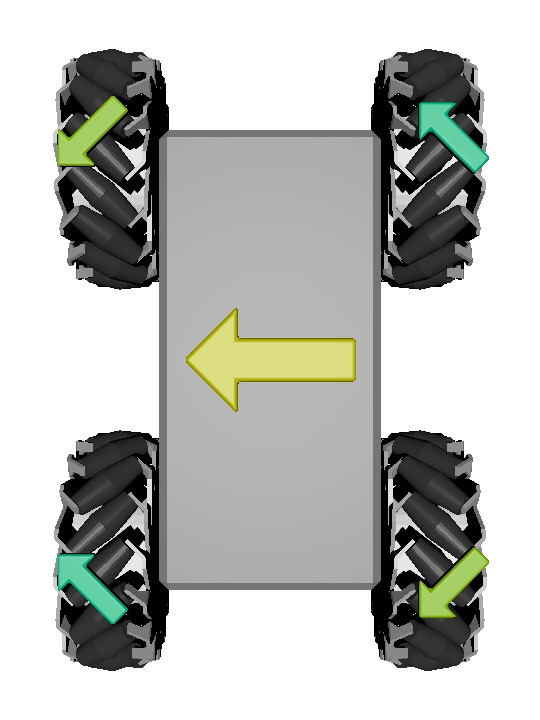
\includegraphics[width=40mm]{Image/ロボット3}
							\\(c)左並進
						\end{center}
						\begin{center}
							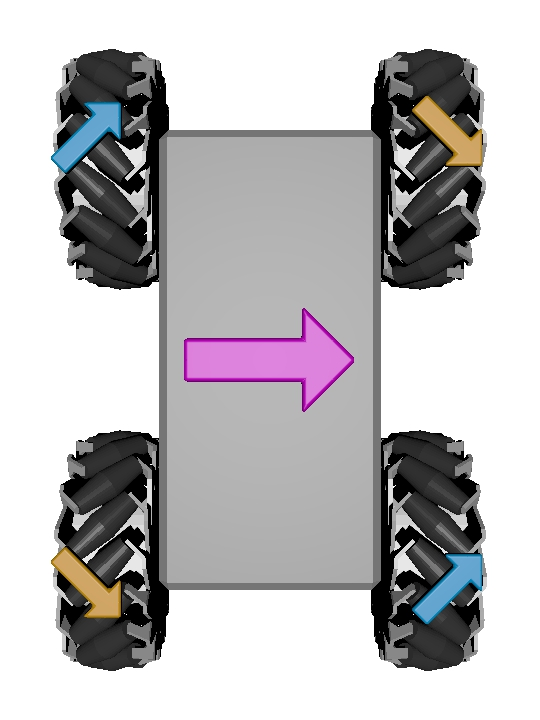
\includegraphics[width=40mm]{Image/ロボット4}
							\\(d)右並進
						\end{center}
					\end{minipage}
					\begin{minipage}{0.33\hsize}
						\begin{center}
							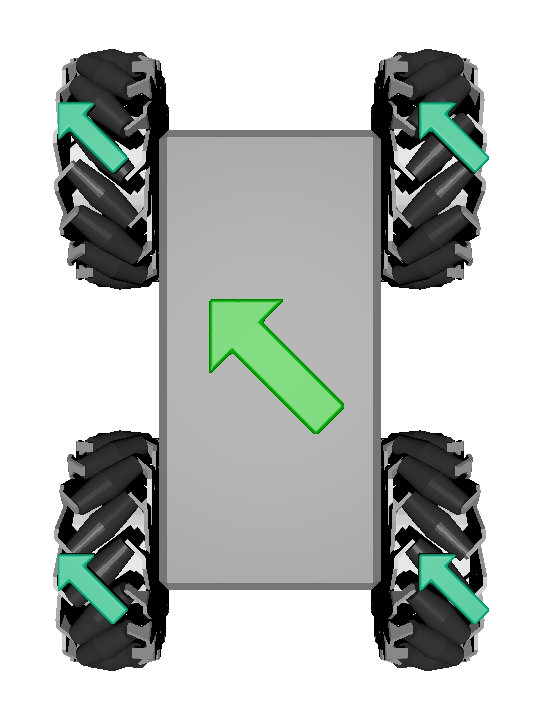
\includegraphics[width=40mm]{Image/ロボット5}
							\\(e)左斜め移動
						\end{center}
						\begin{center}
							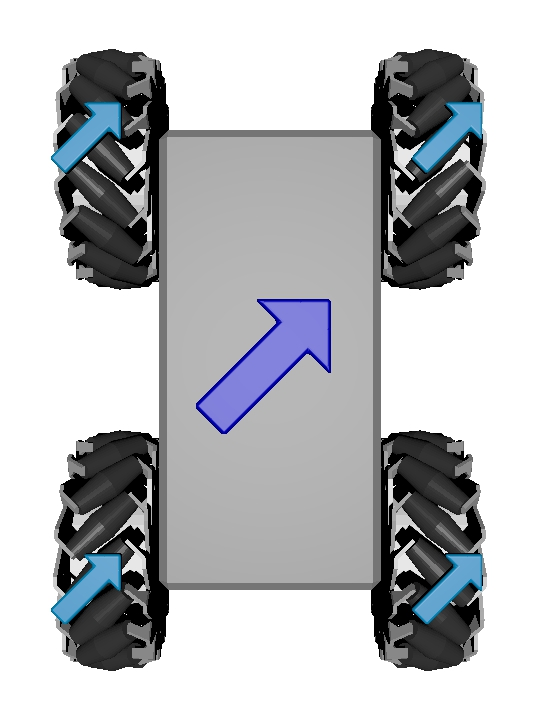
\includegraphics[width=40mm]{Image/ロボット6}
							\\(f)右斜め移動
						\end{center}
					\end{minipage}
				\end{tabular}
				\caption{車輪のベクトルと本体の進行方向}
				\label{移動系}
			\end{center}
		\end{figure}

	\section{操作プログラム}
	ここではメカナムホイールの回転数を制御する計算式や、そのために必要な定義などを説明する。

		\subsection{定義}
		メカナムホイールを操作するためには縦方向、横方向、回転方向の3種類の値が必要である。さらにこれらを計算してPWM値とするため、アナログ値を出力できるコントローラでなければならない。そのため、これらの基準を満たしているDualShock3を用いて操作する。また、プログラムの処理にはArduinoMegaを使用する。アナログスティックの初期位置を原点とし、そこからX方向とY方向に傾けることで、その量に応じた値が出力される。左スティックは移動用で倒した方向に並行移動することができる。右スティックは旋回用でこちらはX軸の値しか出力しない。アナログスティックの位置を座標化したものを図\ref{座標}に示す。

		\begin{figure}[htp]
			\begin{center}
				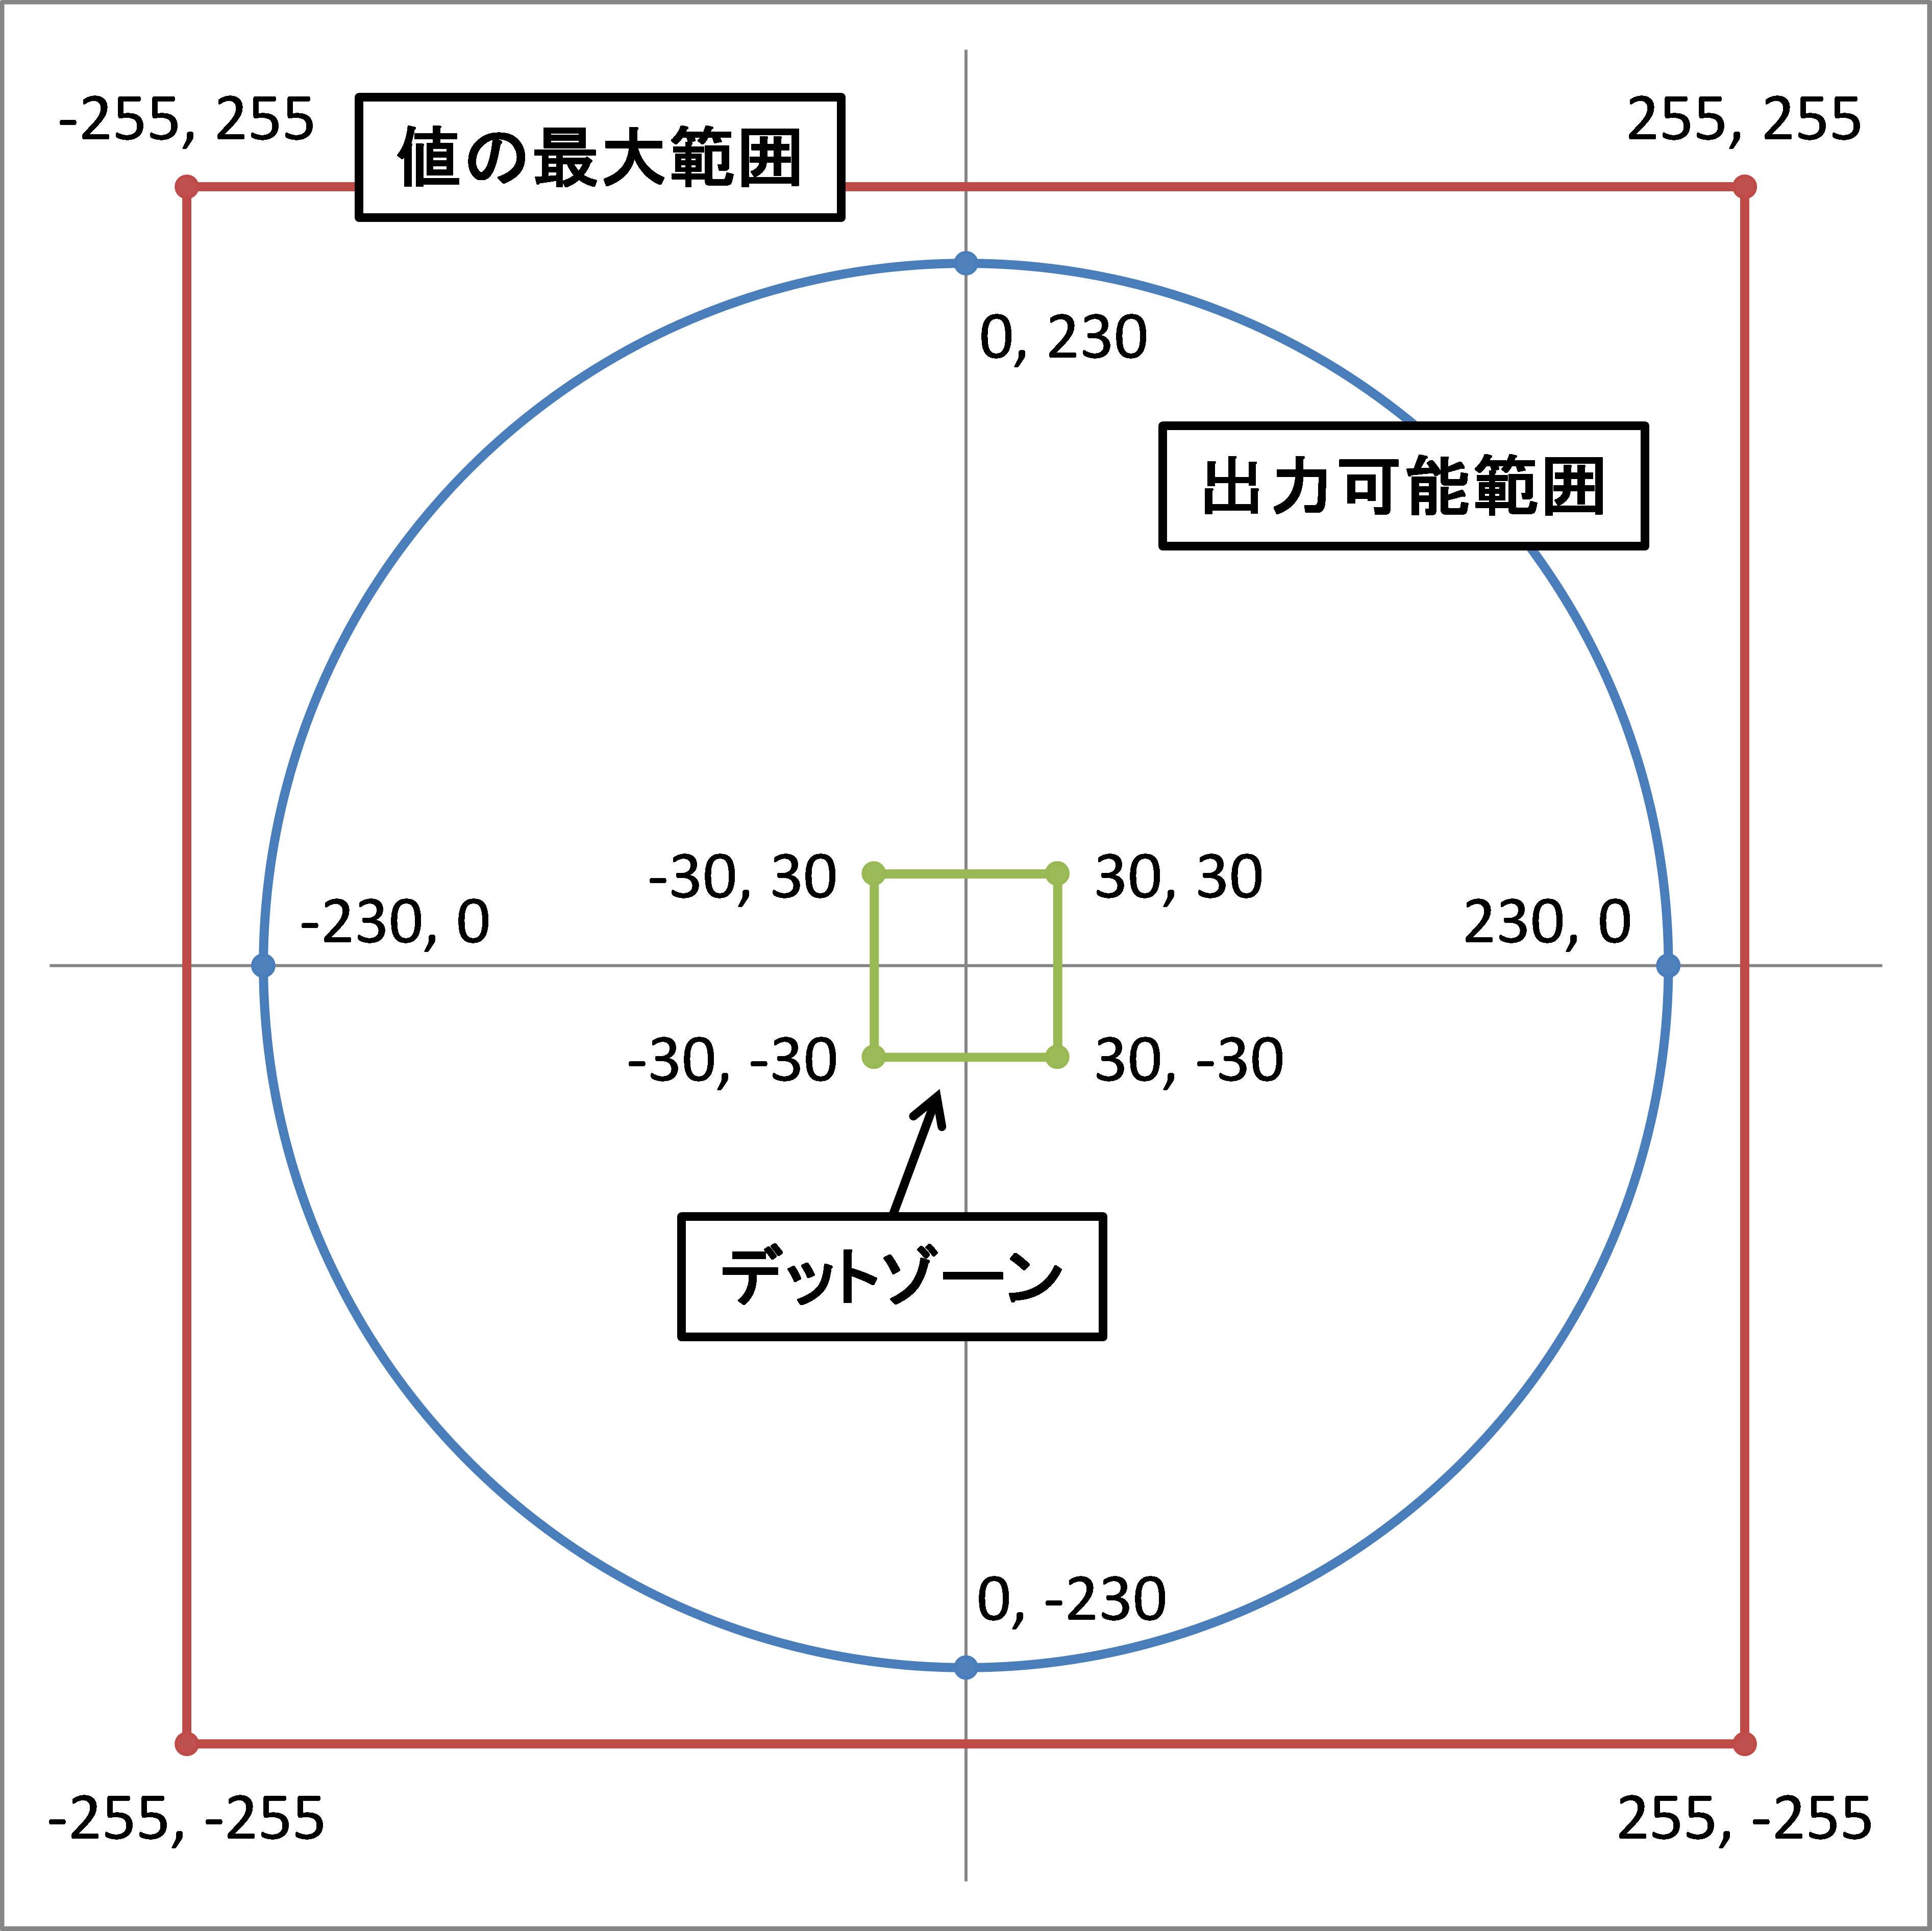
\includegraphics[width=100mm]{Image/座標.png}
				\caption{アナログスティックの座標}
				\label{座標}
			\end{center}
		\end{figure}

		\subsection{計算式}
		左スティックはY方向に傾けることで$L_y$、X方向に傾けることで$L_x$を出力する。右スティックはX方向に傾けることで$R_x$を出力する。図\ref{対角}の番号をメカナムホイールに取り付けられたモータの番号とすると、PWM値の計算式は以下のようになる。

		\begin{eqnarray}
		M_1 = L_y + L_x + R_x
		\label{式1}
		\\
		M_2 = L_y - L_x + R_x
		\label{式2}
		\\
		M_3 = L_y - L_x + R_x
		\label{式3}
		\\
		M_4 = L_y + L_x + R_x
		\label{式4}
		\end{eqnarray}

\chapter{今回製作したロボットのメカナムホイールの問題点}

	\section{問題点}

	\begin{itemize}
		\item 直進中の環境によって進行方向がずれてしまい斜めに進んでしまう。
		\item 駆動開始時に右方向に大きくずれることがある。
		\item 停止時に慣性で右方向にずれる。
	\end{itemize}
	\label{問題点}

	\section{原因}

		\subsection{項目}
		以下に\ref{問題点}の問題点が発生すると思われる原因を示す。

		\begin{enumerate}
			\item ロボットの重心
			\item 加工精度(タイヤの設置位置)
			\item モータ個々の差
			\item モータドライバの差
		\end{enumerate}

		\subsection{影響を及ぼしている原因とその理由}
		問題の中で一番影響を及ぼしているのはロボットの重心問題である。理由は、図\ref{積込ロボット重心}に示すように積み込みロボットには、正面に箱を積み上げるためのラックハンド、片方の側面に箱を回収するためのサイドアームが取り付いているため、重心の位置が中心よりも右前にずれている。これにより左後ろのタイヤが浮くことがあり、4輪全体が均等に力を床に伝えきれないことから直進中にロボットの進行方向が左右に傾き、ずれてしまうことが問題なのである。

		\begin{figure}[htp]
			\begin{center}
				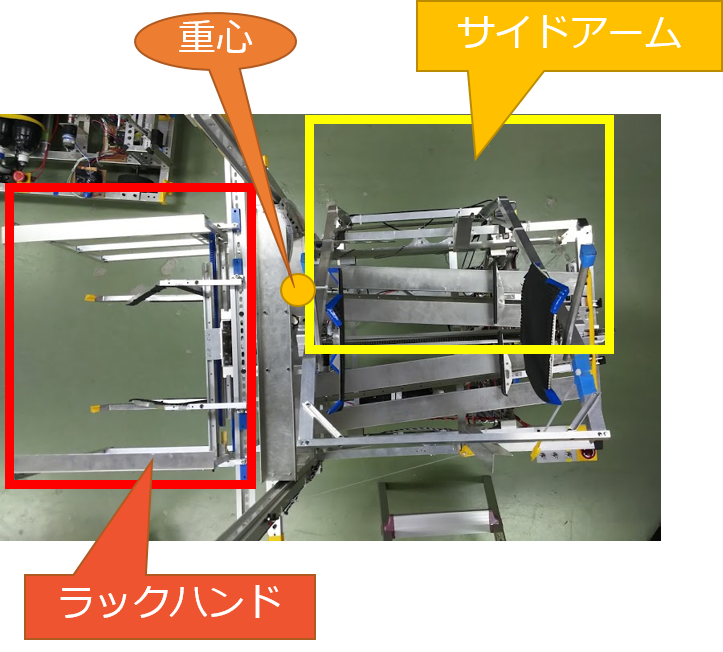
\includegraphics[width=100mm]{Image/積込ロボット重心.png}
				\caption{積み込みロボット重心}
				\label{積込ロボット重心}
			\end{center}
		\end{figure} 

	\section{方向自動修正}
	ロボットの進行中の傾きによって直進ができない為、図\ref{Arduino9軸モーションシールド図}のArduino 9軸モーションシールドに搭載されているジャイロセンサを使用し改善を行った。

\begin{figure}[htp]
		\begin{center}
			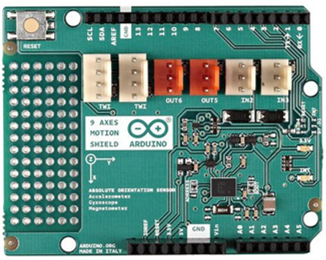
\includegraphics[width=40mm]{Image/Arduino9軸モーションシールド図.png}
			\caption{Arduino9軸モーションシールド図}
			\label{Arduino9軸モーションシールド図}
		\end{center}
\end{figure}

		\subsection{ジャイロセンサ}
		ジャイロセンサとは、角速度センサとも呼ばれ、角度が単位時間当たりにどれだけ変化しているのか計測できるセンサである。このセンサは身近にも用いられており、ドローンのバランス調整やPS4のコントローラに使われている。

		\subsection{補正方法}
		今回使用したプログラムではジャイロセンサから得られた角度を判定して0°からずれた分を補正値のPWM値としてメカナムホイールの動作で使用した式\ref{式1},\ref{式2},\ref{式3},\ref{式4}にerrの形で代入することで以下の式となる。

\begin{eqnarray}
M_1 = L_y + L_x + R_x + err
\\
M_2 = L_y - L_x + R_x + err
\\
M_3 = L_y - L_x + R_x + err
\\
M_4 = L_y + L_x + R_x + err
\end{eqnarray}

こうすることでコントローラからの信号入力中や停止時に慣性で曲がった場合も補正が自動で行われて方向修正が可能となる。

	\section{補正の効果}
	補正制御あり、なしを比較するため実験を行う。

		\subsection{実験方法}
		学校の廊下の距離10m、幅約2.8mをPWM値230、200、150、100、50の5種類で直進させ、そのずれ幅を5回測定し平均値で比較する。廊下の壁に接触した場合その時点のずれ幅と進行距離を計測する。

		\subsection{実験結果}
		
		補正制御実験の結果から得られた記録を表\ref{1}、表\ref{2}に示す。この時、右方向のずれを正、左方向のずれを負とする。その比較をグラフとして図\ref{図3}に示す。
補正なしの場合、全体が左方向に1m前後と大きく傾く結果となった。PWM値が小さいほど外側にずれて、大きいほど内側にずれた。
補正ありの場合、補正なしのようなずれを小さくできたがPWM値の大きさによって左右にずれが発生する結果となった。PWM値が大きいほど左にずれ、PWM値が小さいほど右にずれる。ずれ幅は中心から左右とも0.4m以内に収まった。
補正ありの時に右方向にずれた理由は、速度が遅く、補正が効きやすくなっていたがロボットの右前に重心がある問題から正面を向いたまま並行に移動してしまった為、傾きが検出できず徐々に右に進んでしまう結果になったと考えられる。速度が速い時に左にずれた理由は直進のPWM値が大き過ぎて補正のPWM値が負けてしまい制御なしの時と同様に左方向に引っ張られたと考えられる。

		\begin{table}[htb]
			\begin{center}
				\caption{補正なしの表}
				\label{1}
				\begin{tabular}{|c|c|c|c|c|c|c|c|c|c|c|} \hline
					& \multicolumn{10}{c|}{PWM値} \\ \cline{2-11}
					回数 & \multicolumn{2}{c|}{230}
					& \multicolumn{2}{c|}{200}
					& \multicolumn{2}{c|}{150}
					& \multicolumn{2}{c|}{100}
					& \multicolumn{2}{c|}{50} \\ \cline{2-11}
					& 距離 & ずれ幅 & 距離 & ずれ幅 & 距離 & ずれ幅 & 距離 & ずれ幅 & 距離 & ずれ幅 \\ \hline
					1 & 8.00 & -0.52 & 10.0 & -0.66 & 6.80 & -0.72 & 6.70 & -0.72 & 6.50 & -0.70 \\
					2 & 8.50 & -0.73 & 10.0 & -0.73 & 7.20 & -0.73 & 6.20 & -0.66 & 8.80 & -0.68 \\
					3 & 7.80 & -0.77 & 10.0 & -0.77 & 7.10 & -0.73 & 5.70 & -0.66 & 6.00 & -0.66 \\
					4 & 8.00 & -0.72 & 8.50 & -0.80 & 6.80 & -0.66 & 5.90 & -0.72 & 6.30 & -0.73 \\
					5 & 7.80 & -0.71 & 8.90 & -0.64 & 8.80 & -0.66 & 6.10 & -0.72 & 6.00 & -0.73 \\ \hline
					平均 & 8.02 & -0.69 & 9.48 & -0.72 & 7.34 & -0.70 & 6.12 & -0.70 & 6.72 & -0.70 \\ \hline
				\end{tabular}
			\end{center}
		\end{table}

		\begin{table}[htb]
			\begin{center}
				\caption{補正ありの表}
				\label{2}
				\begin{tabular}{|c|c|c|c|c|c|} \hline
					& \multicolumn{5}{c|}{PWM値} \\ \cline{2-6}
					回数 & 230 & 200 & 150 & 100 & 50 \\ \hline
					1 & -0.14 & -0.40 & -0.11 & -0.01 & 0.26 \\
					2 & -0.10 & -0.40 & 0.07 & 0.18 & 0.31 \\
					3 & -0.32 & -0.11 & 0.13 & 0.16 & 0.37 \\
					4 & -0.40 & -0.58 & 0.16 & 0.14 & 0.28 \\
					5 & -0.56 & -0.54 & 0.05 & 0.17 & 0.24 \\ \hline
					平均 & -0.30 & -0.40 & 0.06 & 0.13 & 0.29 \\ \hline
				\end{tabular}
			\end{center}
		\end{table}

		\begin{figure}[htp]
			\begin{center}
				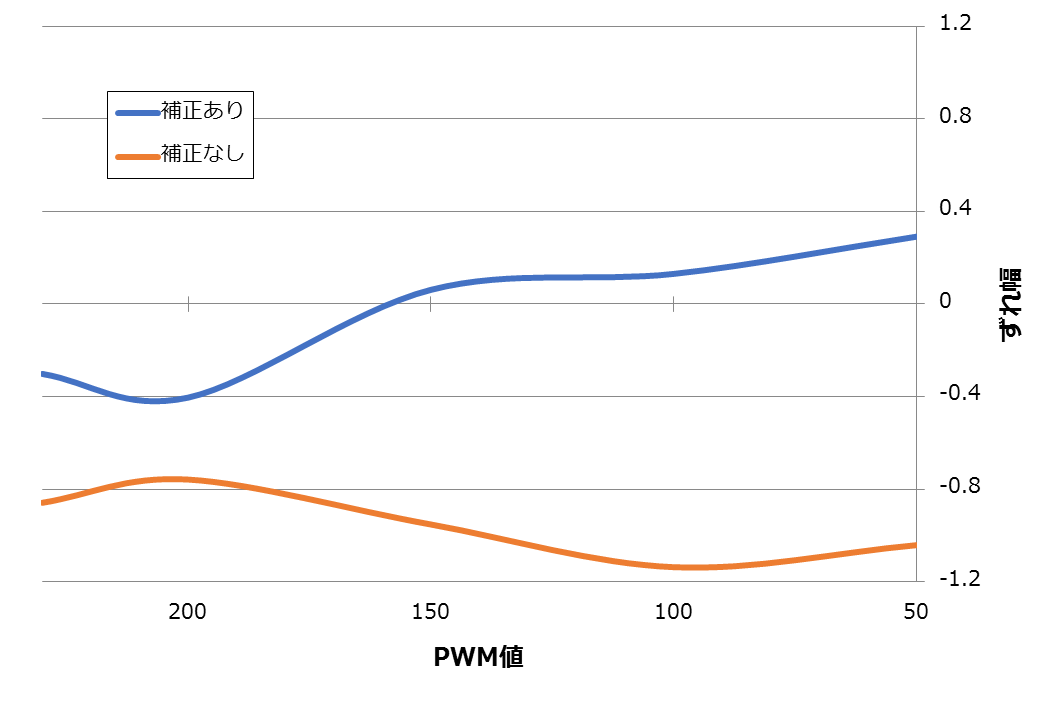
\includegraphics[width=120mm]{Image/図3.png}
				\caption{比較のグラフ}
				\label{図3}
			\end{center}
		\end{figure}

%%%%%%%%%%%%%%%%%%%%%%%%%%%%%%%%%%%%%%%%%%%%%%%%%%%%%%%%%%%%%%%%
\chapter{おわりに}
実験結果からジャイロセンサでの補正効果は見られたがロボットの傾き情報のみでは、ロボットが正面を向いたまま少しずつ斜めに進行した際に補正の対応ができないことと、直進のPWM値が補正のPWM値を大きく上回る場合、補正効果が薄れてしまうことから完璧な補正はすることができなかった。今後の課題として、ジャイロセンサ以外のセンサを用いて傾き以外の画像や位置といった情報を取り込み、直進のPWM値と比例して補正のPWM値を調整できる制御ができればより良い補正が可能となると考える。

% 参考文献
\begin{thebibliography}{1}
\bibitem{gyro} Arduino9AxesMotionLibrary,http:{\slash}{\slash}www.arduino.org{\slash}learning{\slash}reference{\slash}9-axes-motion,2017{\slash}01{\slash}16閲覧
\end{thebibliography}

\chapter*{謝辞}
\addcontentsline{toc}{chapter}{謝辞}
本研究を進めるにあたり、ご指導を頂いた卒業論文指導教員の伊藤恒平先生、伊勢大成先生、また、大会まで多くの応援や差し入れなどをしていただいた皆様へ心から感謝の気持ちと御礼を申し上げたく、謝辞にかえさせていただきます。

\chapter*{付録}
\appendix
\lstinputlisting[caption=メカナムホイールの操作とジャイロによる方向修正プログラム,label=mecanum]{PS3BT_tumihakobi_3jiku_5.ino}

%%%%%%%%%%%%%%%%%%%%%%%%%%%%%%%%%%%%%%%%%%%%%%%%%%%%%%%%%%%%%%%%
\end{document}

